\subsection{饱和与过饱和}
与溶质固相处于平衡状态的溶液称该物质的饱和溶液。溶解度曲线实际上给出不同温度下的饱和溶液的浓度,所以溶解度曲线也称为饱和曲线。在一定条件下,对给定的物质,这条曲线是确定的,可以通过准确测定物质在不同温度下的溶解度绘制出来。

\begin{figure}[hbp]
 \centering
 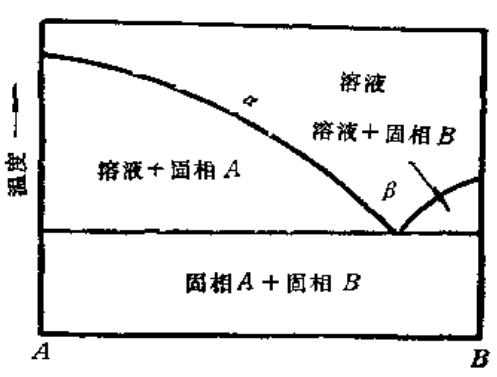
\includegraphics[width=0.5\textwidth]{fig/cp03/img3.5.jpg}
 \caption{二元体系相图,$\alpha\beta$为从溶液中生长晶体的区域。}
\end{figure}

\begin{figure}[htpb]
 \centering
 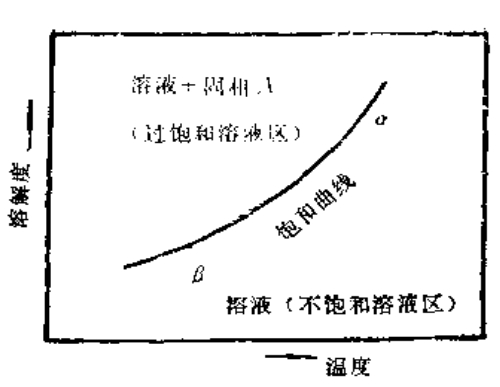
\includegraphics[width=0.5\textwidth]{fig/cp03/img3.6.jpg}
 \caption{饱和曲线(溶解度曲线)。}
\end{figure}
如果A为溶质,B为溶剂,A与B之间也不形成任何化合物,则图3.6中的溶解度曲线就是图3.5中液相线的一部分$\alpha\beta$。图3.6中曲线$\alpha\beta$的下部是不饱和溶液区,$\alpha\beta$的上方是固相和溶液共存区。当溶液状态进入该区时,应当结晶出固相A,此时的溶液浓度应为在该温度下和固相A相平衡的饱和溶液的浓度。但实际上,这样的溶液常常不析出晶体。这种所含溶质量比在同一条件下饱和溶液中所含溶质量要多的溶液称为过饱和溶液。凡是状态点处在饱和曲线以上区域内的溶液都是过饱和溶液,所以这个区域也称为过饱和溶液区。

溶液都具有程度不同的过饱和现象。过饱和状态是从溶液中生长晶体的前提条件,因此从上一世纪以来就对过饱和溶液进行了较深人的研究。

过饱和状态在热力学上是不稳定的,整个过饱和区的不稳定程度也是不一样的。溶液状态靠近饱和曲线就较为稳定,离饱和曲线越远就越不稳定。1897年Ostwald首先引入“不稳过饱和” 和“亚稳过饱和”的概念。他把在无晶核存在的情况下能自发析出固相的过饱和溶液称为“不稳过饱和”溶液,而把不能自发结晶的过饱和溶液称为“亚稳过饱和”溶液。

随后,Miers对自发结晶和过饱和度之间的关系进行了广泛的研究。他测量了许多盐类的浓溶液在冷却过程中折射率的变化,试图找出过饱和溶液中不稳区和亚稳区的界限。他的实验结果可用图3.7来表示,图中除了溶解度曲线外,在其上方还有一条溶液开始自发结晶的界限,称为过溶解度曲线.这条曲线将过饱和溶液分为亚稳区和不稳区。过溶解度曲线不像溶解度曲线那样确定,极易受一些外界因素(如溶液搅拌程度)影响。关于这一观点引起了很大争论,有的人认为不可能存在这样一条使溶液性质突然起变化的曲线,有的人则倾向于把过溶解度曲线看成是位于过饱和区的一个区域或窄带。

\begin{figure}[htb]
 \centering
 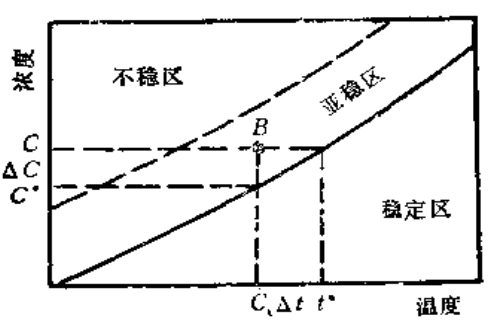
\includegraphics[width=0.5\textwidth]{fig/cp03/img3.7.jpg}
 \caption{溶液状态图}
\end{figure}

但是不论过溶度曲线是否真实存在,但在过饱和区,靠近溶解度曲线确实存在亚稳区,这个事实是毋庸置疑的。整个温度-浓度图还是可分成稳定区、亚稳区和不稳区三个区域,其中稳定区是确定的,而亚稳区和不稳区在一定程度上是可变的,很难严格区分。这些区域的特征如下:

稳定区:即不饱和区,不可能发生结晶作用。

亚稳(过饱和)区:处于这个区域的溶液不会自发地发生结晶作用。如将籽晶放人处于亚稳区的溶液中,晶体就会在籽晶上生长。

不稳(过饱和)区:处于这个区域的溶液会自发地发生结晶作用。

三个区域以亚稳区最为重要,因为从溶液中生长晶体都是在这个区域内进行的。从培养单晶的角度出发,我们总希望析出的溶质都在籽晶上逐渐生长而不希望中出现自发晶体(即杂晶),为此要求在整个生长过程中使溶液状态始终保持在亚稳区内。亚稳区虽无法精确测量, 但其大小、趋向还是可以用过饱和度(或过冷度)来估计的。亚稳区的大小既同结晶物质的本性有关,也极易受外界条件的影响, 如搅拌、振动、温度、杂质等。不同物质溶液的亚稳区差别相当大(见表3.2)。过饱和度有以下几种表示方式:
\begin{eqnarray}
&& \text{浓度驱动力}\ \Delta c,\quad\Delta c=c-c^*; \\
&& \text{过饱和比}\ s,\quad s=\frac{c}{c^*}; \\
&& \text{过饱和度或相对过饱和度}\ \sigma,\quad\sigma=\frac{\Delta c}{c^*}=s-1,
\end{eqnarray}
其中$c$是溶液的实际浓度,$c^*$是溶液在同一温度下的平衡饱和浓度(图3.7)。在以上三种表示方式中,只有是有量纲的(用摩尔分数表示是例外),其数值随浓度表示方式的不同而差别很大,但对$s$和$\sigma$的影响却不很明显(表3.1)。表示过饱和度时,必须注明溶液温度,因为溶液的平衡饱和浓度是随温度的变化而变化。

%TODO: 表3.1 3.2
(表3.1)(表3.2)

过饱和度也可用温度来表示。若将某一物质在$t^*$℃时,将其饱和溶液冷却至$t$℃,溶液进入过饱和状态,如果没有结晶析出,则该溶液的过饱和度为$\Delta t=(t^*-t)$(见图3.7),这实际上就是溶液的过冷度(在单组分体系中,只用过冷度而不使用过饱和度这个名词)。一些盐类水溶液的最大可容许过冷度列于表3.2中。这些数据是将25℃的饱和溶液在有晶体存在和适当搅拌的情况下,通过缓慢降温测得的。虽然在实验室条件下测得的过冷度和生产实践中的情况有较大差别,但也可以作为对在该实验条件下比较不同物质溶液亚稳区大小的量度。过冷度和过饱和度的关系为
\begin{equation}
\Delta c = \left(\frac{dc^*}{dt}\right)\Delta t.
\end{equation}
